\section{\lr{word2vec}}
به منظور آموزش بردارها از جملات تمیز شده 6 ژانری که بیشترین تعداد جملات را داشتند استفاده شده است. کد استفاده شده مربوط به تمرین 
\textit{a2}
است که برای هر ژانر داده مربوطه جایگزین شده است. 

برای تحلیل و مقایسه بردارهای ژانرها، ابتدا کلمات مشترک بین این 6 ژانر استخراج می شوند سپس شباهت کسینوسی بردارها محاسبه می شود. کد این بخش در فایل
\texttt{compare.py}
قرار دارد. در مجموع 11146 کلمه مشترک بین ژانرها وجود دارد که تعدادی از آنها در ادامه بررسی شده اند.
در شکل \ref{fig11} شباهت کسینوسی بردارهای کلمه attacker بین ژانرها مقایسه شده است. در این بین ژانرهای
Drama
و
Romance
بیشترین شباهت را به هم دارند. دلیل آن می تواند ظاهر شدن این کلمه در context مشابه در داده هر دو ژانر باشد. همچنین
Fantasy
و
Romance
کمترین شباهت را دارند که می تواند حاصل از تفاوت context این کلمه در داده این ژانرها باشد. 
 \begin{figure}[H]
	\centering
	
	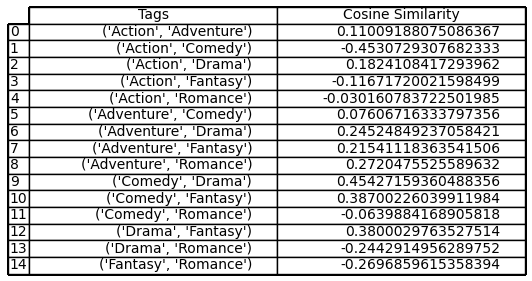
\includegraphics[width=1\textwidth,height=1\textheight,keepaspectratio]{../report/word2vec/attacker}
	\caption{شباهت کسینوسی بردارهای کلمه attacker}
	\label{fig11}
	
\end{figure} 

در شکل 
\ref{fig12}
شباهت کسینوسی بردارهای کلمه
everyone
مقایسه شده است. انتظار می رود که این کلمه تقریبا برای همه ژانرها بردار مشابهی داشته باشد؛ اما بردار این کلمه بین ژانرهای 
\texttt{Action-Fantasy}،
\texttt{Action-Romance}
و
\texttt{Comedy-Drama}
تفاوت دارد. این تفاوت می تواند ناشی از تفاوت در context کلمه در داده این ژانرها یا کوچک بودن بردارها و کم بودن اطلاعات آنها باشد.
 \begin{figure}[H]
	\centering
	
	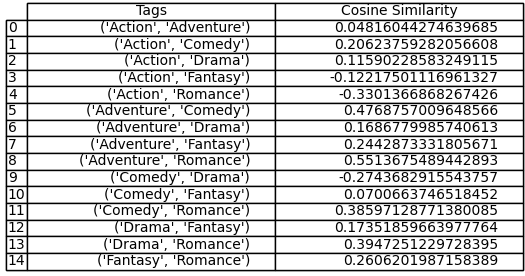
\includegraphics[width=1\textwidth,height=1\textheight,keepaspectratio]{../report/word2vec/everyone}
	\caption{شباهت کسینوسی بردارهای کلمه everyone}
	\label{fig12}
	
\end{figure} 



نکته مهم این است طول این بردارها 10 است. به همین دلیل اطلاعات زیادی را در خود ذخیره نمی کنند و دلیل برخی شباهت ها یا تفاوت های در از انتظار نیز همین است. 